Synchronizing with the server after being offline is fairly simple for the client provided that it kept some sort of queue for the edits it made while offline, and the edit id of the last edit it received from the server. The client will use the \hyperref[sec:message:push]{push} command with all of it’s queued edits and the cached edit id to synchronize itself with the server. The next update it receives will be the merged version of the spreadsheet.

\begin{figure}[H]
    \begin{center}
        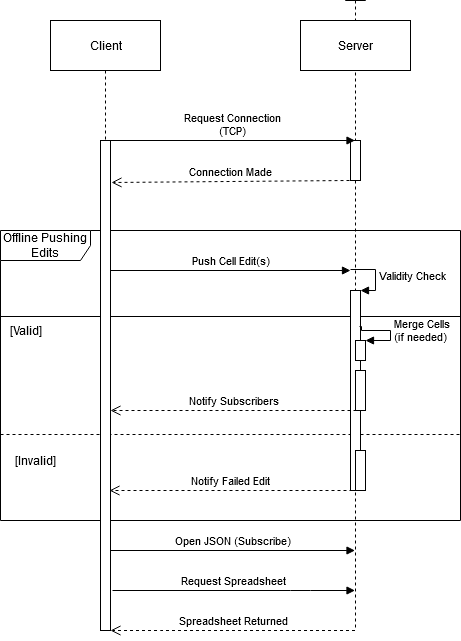
\includegraphics[width=2.5in]{Figures/OfflineWithEdits.png}
        \caption{Synchronizing sequence}
    \end{center}
\end{figure}